Decomposition is a mathematical technique to convert a large-base number into a mathematical formula expressing the same value in a smaller base. This section will explain number decomposition and polynomial decomposition. 

\subsection{Number Decomposition}
\label{subsec:number-decomp}
We fix a modulus $q\ge 2$ and write $\mathbb{Z}_q=\mathbb{Z}/q\mathbb{Z}$. Let $\gamma\in\mathbb{Z}_q$. Number decomposition expresses $\gamma$ as a sum of multiple numbers in base $\beta$ as follows: 

$ $

$\gamma = \gamma_1 \dfrac{q}{\beta^1} + \gamma_2 \dfrac{q}{\beta^2} + \cdots + \gamma_\ell \dfrac{q}{\beta^\ell}  $

$ $

\noindent where $\beta\ge 2$ is a base and $\ell\ge 1$ the decomposition level. We assume $\beta^\ell \mid q$ and take digits $\gamma_i\in\{0,1,\ldots,\beta-1\}$, under these conditions the decomposition is unique. This is visually shown in \autoref{fig:decomp}. (If $\beta^\ell\nmid q$, see \autoref{subsec:approx-decomp}.) 
Each $\gamma_i$ represents a base-$\beta$ digit at position $i$. When $q$ is a power of two, this corresponds to a shift by $i\cdot \log_2\beta$ bits.

\begin{figure}[h!]
    \centering
  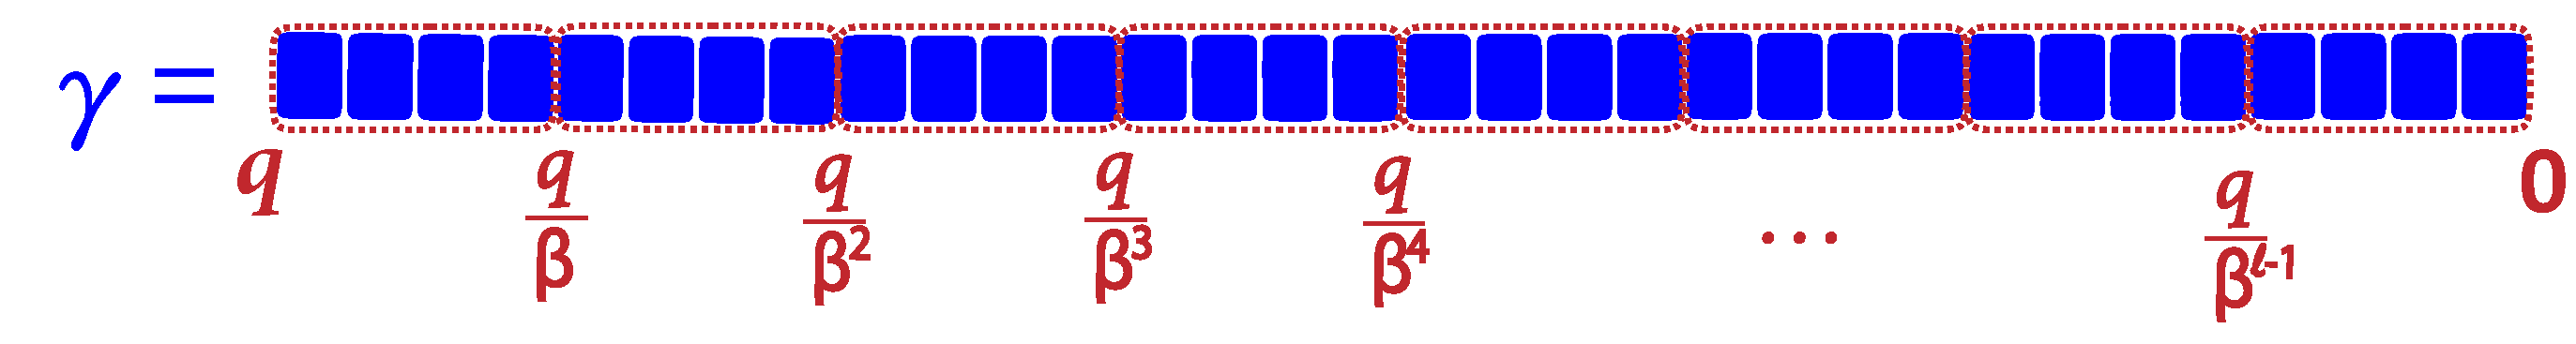
\includegraphics[width=0.8\linewidth]{figures/decomp.pdf}
  \caption{An illustration of number decomposition.}
  \label{fig:decomp}
\end{figure}

We define the decomposition of number $\gamma$ into base $\beta$ with level $\ell$ as follows:


$ $

$\textsf{Decomp}^{\beta, \ell}(\gamma) = (\gamma_1, \gamma_2, \text{ } \cdots , \text{ } \gamma_\ell)$.
 
$ $

Number decomposition is also called radix decomposition, where the base $\beta$ is called a radix. 


\subsubsection{Example}

Suppose we take $\gamma=13$ in $\mathbb{Z}_{16}$. Suppose we want to decompose 13 with the base $\beta = 2$ and level $\ell = 4$. Then, 13 is decomposed as follows:

$ $

$13 = 1 \cdot \dfrac{16}{2^1} + 1 \cdot \dfrac{16}{2^2} + 0 \cdot \dfrac{16}{2^3} + 1 \cdot \dfrac{16}{2^4}$

$ $

$\textsf{Decomp}^{2, 4}(13) = (1, 1, 0, 1)$


\subsection{Polynomial Decomposition}
\label{subsec:poly-decomp}

This time, suppose we have polynomial $f$ in the polynomial ring ${\mathbb{Z}_q[x] / (x^n + 1)}$. Therefore, each coefficient $c_i$ of $f$ is an integer modulo $q$. Polynomial decomposition expresses $f$ as a sum of multiple polynomials in base $\beta$ and level $\ell$ as follows:


\begin{tcolorbox}[title={\textbf{\tboxlabel{\ref*{subsec:poly-decomp}} Polynomial Decomposition}}]

Given $f\in \mathbb{Z}_q[x]/(x^n+1)$, fix $\beta\ge 2$ and $\ell\ge 1$ with $\beta^\ell\mid q$. We write

$ $

$
f=\sum\limits_{i=1}^{\ell} f_i\,\dfrac{q}{\beta^i}, \qquad f_i\in \mathbb{Z}_q[x]/(x^n+1)
$

$ $

where each $f_i$ is obtained by decomposing every coefficient of $f$ in base $\beta$. If $f=\sum\limits_j c_j x^j$ with $c_j\in\mathbb{Z}_q$, then
$c_j=\sum\limits_{i=1}^{\ell} c_{j,i}\,\dfrac{q}{\beta^i}$ with $c_{j,i}\in\{0,\ldots,\beta-1\}$,
and $f_i=\sum_j c_{j,i} x^j$.
We denote the decomposition of the polynomial $f$ into the base $\beta$ with the level $\ell$ as follows:

$ $

$\textsf{Decomp}^{\beta, \ell}(f) = (f_1, f_2, \text{ } \cdots , \text{ } f_\ell)$
 $ $
\end{tcolorbox}




\subsubsection{Example}

Suppose we have the following polynomial in the polynomial ring $\mathbb{Z}_{16}[x] / (x^4 + 1)$:

$ $

$f = 6x^3 + 3x^2 + 14x + 7 \in \mathbb{Z}_{16}[x] / (x^4 + 1)$

$ $

Suppose we want to decompose the above polynomial with base $\beta = 4$ and level $\ell = 2$. Then, each degree's coefficient of the polynomial $f$ is decomposed as follows:

$ $

${\bm{x}^{\bm{3}}}$: $6 = \color{blue}{1 \cdot \dfrac{16}{4^1}} \color{black}+ \color{red}{2 \cdot \dfrac{16}{4^2}}$

${\bm{x}^{\bm{2}}}$: $3 = \color{blue}{0 \cdot \dfrac{16}{4^1}} \color{black}+ \color{red}{3 \cdot \dfrac{16}{4^2}}$

${\bm{x}^{\bm{1}}}$: $14 = \color{blue}{3 \cdot \dfrac{16}{4^1}} \color{black}+ \color{red}{2 \cdot \dfrac{16}{4^2}}$

${\bm{x}^{\bm{0}}}$: $7 = \color{blue}{1 \cdot \dfrac{16}{4^1}} \color{black}+ \color{red}{3 \cdot \dfrac{16}{4^2}}$

$ $

The decomposed polynomial is as follows:

$f = 6x^3 + 3x^2 + 14x + 7 = \color{blue}{(1x^3 + 0x^2 + 3x + 1) \cdot \dfrac{16}{4^1}} \color{black}+ \color{red}{(2x^3 + 3x^2 + 2x + 3) \cdot \dfrac{16}{4^2}} \color{black}$

$ $

$\textsf{Decomp}^{4, 2}(6x^3 + 3x^2 + 14x + 7) = (1x^3 + 0x^2 + 3x + 1, 2x^3 + 3x^2 + 2x + 3)$

\subsubsection{Discussion}

Note that after decomposition, the original coefficients of the polynomial got reduced to smaller numbers. This characteristic is importantly used in homomorphic encryption's multiplication, for reducing the growth rate of the noise. Normally, the polynomial coefficients of ciphertexts are large because they are uniformly random numbers. Reducing such big constants is important to reduce the noise growth during homomorphic multiplication. We will discuss this more in detail in \autoref{subsec:tfhe-mult-cipher}.


\subsection{Approximate Decomposition}
\label{subsec:approx-decomp}

\begin{figure}[h!]
    \centering
  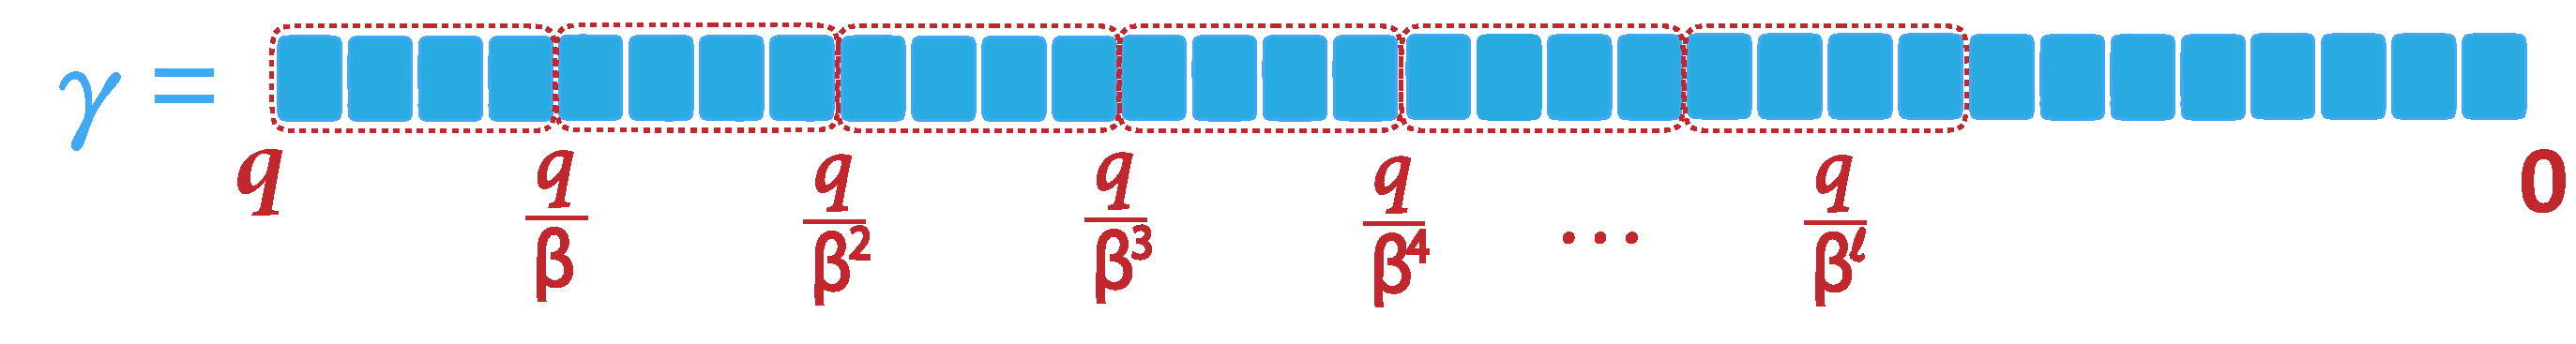
\includegraphics[width=0.7\linewidth]{figures/decomp3.pdf}
  \caption{An illustration of approximate decomposition}
  \label{fig:decomp3}
\end{figure}

If no level $\ell$ satisfies $\beta^\ell \mid q$, then some lower bits of $q$ must be discarded during decomposition, as shown in \autoref{fig:decomp3}. Such lower bits can be rounded to the nearest multiple of $\dfrac{q}{\beta^\ell}$ during decomposition. In such a case, the decomposition is an approximate decomposition. 
Formally, when $\beta^\ell\nmid q$ we can write
$$
\gamma=\sum_{i=1}^{\ell}\gamma_i\,\frac{q}{\beta^{i}}+\varepsilon,\qquad
\gamma_i\in\{0,\ldots,\beta-1\},\quad
|\varepsilon|\le \frac{q}{2\beta^{\ell}}
$$
(using nearest-integer rounding and identifying $\gamma$ with its integer representative). The polynomial case is analogous, coefficient-wise.



\subsection{Gadget Decomposition}
\label{subsec:gadget-decomposition}

Gadget decomposition is a generalized form of number decomposition (\autoref{subsec:number-decomp}). In number decomposition, a number $\gamma$ is decomposed as follows: 

$\gamma = \gamma_1 \dfrac{q}{\beta^1} + \gamma_2 \dfrac{q}{\beta^2} + \cdots + \gamma_\ell \dfrac{q}{\beta^\ell} $

$ $

In gadget decomposition, we decompose $\gamma$ as follows: 

$\gamma = \gamma_1 g_1 + \gamma_2 g_2 + \cdots + \gamma_\ell g_\ell $

$ $

We denote $\vec{g} = (g_1, g_2, \cdots, g_\ell)$ as a gadget vector, and $\textsf{Decomp}^{\vec{g}}(\gamma) = (\gamma_1, \gamma_2, \text{ } \cdots , \text{ } \gamma_\ell) $

$ $

Then, $\gamma = \langle \textsf{Decomp}^{\vec{g}}(\gamma), \vec{g} \rangle $

$ $

In the case of number decomposition (\autoref{subsec:number-decomp}), its gadget vector is $\vec{g} = \Bigg(\dfrac{q}{\beta}, \dfrac{q}{\beta^2}, \cdots, \dfrac{q}{\beta^\ell}\Bigg)$.